\chapter{离散系统的校正}

\section{模拟化设计}

\subsection{校正思路}

我们通过以下步骤，采用模拟化校正设计校正环节：
\begin{enumerate}
    \item 根据指标，考虑零阶保持器的影响（零阶保持器在离散化后对系统的影响可以近似为一个惯性环节），用连续系统理论设计校正装置$D(s)$
    \item 对$D(s)$进行离散化，确定数字校正装置的脉冲传递函数$D(z)$
    \item 检查离散控制系统的性能是否满足要求
    \item 写出$D(z)$的差分方程（递推形式），编制程序实现的控制规律
    \item 检验设计的正确性
\end{enumerate}

\subsection{连续控制器的离散化方法}

\subsubsection{阶跃响应不变法}

阶跃响应不变法主要表现为以下的形式：

具有零阶保持其的连续对象在单位阶跃序列$1^{*}(t)$作用下的输出，等于连续对象在单位阶跃信号$1(t)$作用下的输出

\subsubsection{替换法}

替换法的基本思想为：对于给定的连续系统传递函数$D(s)$，设法找到$s$域到$z$域的某种映射关系，它将$s$域的变量映射到$z$平面上，由此得到与连续系统传递函数$D(s)$相对应的离散传递函数$D(z)$，常见的替换法有一阶差分近似和双线性变换，具体方法如下：
\begin{enumerate}
    \item 一阶差分：用一阶差分近似导数：
    \begin{itemize}
        \item 后向差分方程：$s = \frac{1-z^{-1}}{T}$，变换后系统仍然稳定
        \item 前向差分方程：$s = \frac{z-1}{T}$，变换后系统可能不稳定
    \end{itemize}
    \item 双线性变换：$s = \frac{2}{T}\frac{1-z^{-1}}{1+z^{-1}}$
    \item 根匹配法：$s+a \rightarrow 1 - e^{-aT} z^{-1}$，匹配完零极点之后需要确定数字控制器增益$K_z$，可以通过以下的方式确定：
    \begin{itemize}
        \item 使数字控制器与模拟控制器在低频处增益一致
        \item 使某类典型输入下的稳态误差保持一致
        \item 根据题目指定的性能指标要求确定
    \end{itemize}
    \item 冲激响应不变法：$D(z) = Z[D(s)]$
\end{enumerate}

具体举例如下：
\begin{center}
    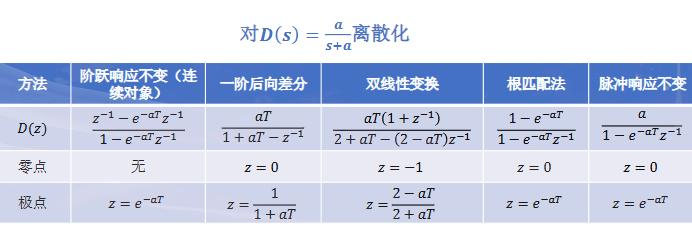
\includegraphics[width = .6\textwidth]{note/discrete system correction/figure/1.png}
\end{center}


\section{离散化设计}

\subsection{设计思路}

离散化的设计采用期望特性校正法，步骤如下：
\begin{center}
    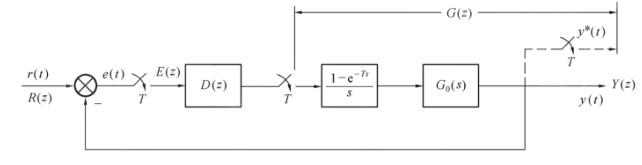
\includegraphics[width = .6\textwidth]{note/discrete system correction/figure/2.png}
\end{center}

一般的单位负反馈系统如下，$D(z)$是我们要设计的校正装置，我们将设计期望的$\Phi(z)$和$\Phi_e(z)$，用以下的式子确定校正装置$D(z)$
\begin{equation*}
    \begin{split}
        \Phi(z) = \frac{G(z)D(z)}{1+G(z)D(z)},&\Phi_e(z) = \frac{1}{1+G(z)D(z)} = 1 - \Phi(z)  \\
        &G(z)D(z) = \frac{\Phi(z)}{\Phi_e(z)} \\
        &D(z) = \frac{\Phi(z)}{\Phi_e(z)G(z)}  \\
    \end{split}
\end{equation*}

同时，在离散化设计的过程中，要遵循\textbf{最少拍设计}，具体为：\textbf{对典型信号能在有限拍内结束过渡过程，同时要在最少的拍内结束过渡过程}

由最小拍设计，我们可以得到以下的几个结论：
\begin{enumerate}
    \item 闭环误差传递函数的形式一定为：$\Phi_e(z) = (1 - z^{-1})^r F(z)$，$r$为输入信号Z变换后分母的关于$1-z^{-1}$的阶次
    \item $E(z) = F(z)A(z)$关于$z^{-1}$的阶次是有限的，且为最小，即$F(z)$关于$z^{-1}$的阶次最小
\end{enumerate}

\subsubsection{广义脉冲传递函数不含纯延迟环节和单位圆上和圆外的零极点}

此时$F(z) = 1$，$\Phi(z) = (1-z^{-1})^r$，$\Phi(z) = 1 - (1 - z^{-1})^r$，在输入为不同的信号的时候得到的调整时间如下表所示：
\begin{center}
    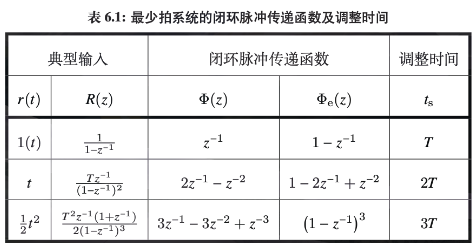
\includegraphics[width = .6\textwidth]{note/discrete system correction/figure/3.png}
\end{center}

\subsubsection{广义脉冲传递函数有纯延迟环节}

此时$G(z) = G_1(z) z^{-L}$，若想要用$D(z)$抵消掉$G(z)$中的纯延迟项，此时$D(z)$会出现超前项，这违背了因果性，在物理上不可实现

所以我们可以得出一个结论：\textbf{若$G(z)$含有纯延迟环节$z^{-L}$，则闭环传递函数$\Phi(z)$也至少包含相同的延迟因子$z^{-L}$}

\subsubsection{广义脉冲传递函数含有单位圆上和圆外的零极点}

若$G(z)$有单位圆上及圆外的零极点，如果不加处理，会造成$D(z)$含单位圆上及圆外的零极点，这样会导致控制器$D(z)$不稳定

所以，我们需要设计$\Phi(z)$和$\Phi_e(z)$，满足以下的要求：
\begin{enumerate}
    \item 闭环传递函数$\Phi(z)$应包含$G(z)$在单位圆上和圆外的零点
    \item 误差传递函数$\Phi_e(z)$应包含$G(z)$在单位圆上和圆外的极点
    \item $\Phi(z)$和$\Phi_e(z)$关于$z^{-1}$的阶次应当相同，且为多项式
\end{enumerate}

\textbf{注意：此设计方法设计出来的校正装置只适用于使用的典型输入信号，对于其他的典型输入信号并不适用！}

\subsubsection{最少拍系统产生纹波的原因}

在经过二拍之后，零阶保持器的输入序列并不是常值脉冲，而是围绕平均值上下波动，从而保持器的输出电压在二拍以后也围绕平均值波动，产生输出纹波。

因此，\textbf{无纹波输出要求序列在有限个采样周期后达到相对稳定}
